\documentclass[titlepage]{article}
\usepackage{babel}
\usepackage{amsmath}
\usepackage{amssymb}
\usepackage{amsthm}
\usepackage{stmaryrd} %ligtning

\usepackage{tabto} %tabulator mit \tab
\usepackage{tikz}
\usetikzlibrary{automata, arrows.meta, positioning, shadows, shapes.geometric} % automaten zeichnen
\usepackage[utf8]{inputenc}
\pagestyle{plain}
\pagenumbering{arabic}
\renewcommand{\arraystretch}{1.3} %vertikaler abstand von tabellen
\usepackage[left=20mm, right=15mm, top=25mm, bottom=7mm, paper=a4paper]{geometry}

\renewcommand{\contentsname}{Inhaltsverzeichnis}
\renewcommand{\]}{\right]}
\renewcommand{\[}{\left[}
\renewcommand{\)}{\right)}
\renewcommand{\(}{\left(}
\renewcommand{\|}{\;|\;}
\newcommand{\n}{\newline}
\renewcommand{\l}{\linebreak}



\begin{document}\begingroup\let\clearpage\relax
	%header
	\begin{center}
	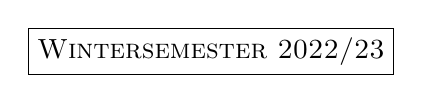
\begin{tikzpicture}
		\draw (0,0) node[draw, rectangle]{\textsc{Wintersemester 2022/23}};
	\end{tikzpicture}
	\hrulefill\\
	\begin{center}
		\LARGE\textsc{Automaten und Berechenbarkeit - Übung 05} \normalsize\\
	\end{center}
	\hrulefill
	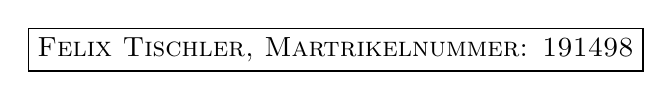
\begin{tikzpicture}
		\draw (0,0) node[draw, rectangle]{\textsc{Felix Tischler, Martrikelnummer: 191498}};
	\end{tikzpicture}
	\date{\today}
\end{center}
	
	\subsection*{Pumping Lemma (PL)}
		Sei $A\in REG$. $\exists n\in\mathbb{N}:\forall x\in A:\mid x\mid>n:x=uvw:$
\begin{enumerate}
	\item $\mid v\mid\ge1$ \\
	\item $\mid uv\mid\le n$ \\
	\item $\forall i\ge0: uv^iw\in A\Leftrightarrow\{u\}\{v\}^*\{w\}\subseteq A$ 
\end{enumerate}
	
	%task one
	\section*{Aufgabe 1}
		Untersuchen Sie, ob die folgenden Sprachen regulär sind oder nicht:
		\subsection*{(a) $A=\{w\mid w\in\{a,b\}^*,\#_a(w)=2\#_b(w)\}$}
			\begin{proof}[Beweis]
	\begin{math}
		Ann:\;A\in REG\Rightarrow\;es\;gilt\;PL\Leftrightarrow\;Sei\;k\;Pumpingzahl:
	\end{math}
	\begin{align*}
		&Wähle\;x=\underbrace{a^{j_1}}_u\underbrace{a^{j_2}}_v\underbrace{a^{2k-j}b^k}_w,j_1+j_2=j,\underbrace{j_2\ge1}_*,\mid x\mid\ge k\\
		&Sei\;x=uvw\;eine\;geiegnete\;Zerlegung\;gemäß\;PL:\\
		&\mid v\mid\ge1\;und\;\mid uv\mid\le n \Rightarrow uv=a^j\mid j\le k\\
		&v^i=a^{{j_2}^i}\\
		&\overset{i=0}{\Longrightarrow} x=a^{j_1}a^{{j_2}^0}a^{2k-j}b^k=a^{j_1}\lambda a^{2k-j}b^k=\underbrace{a^{2k-j_2}b^k}_x\overset{*}{\Rightarrow}x\notin A\quad\lightning
	\end{align*}
\end{proof}
		\subsection*{(b) $B=\{0^n10^m\mid n>m\}$}
			\begin{proof}[Beweis]
	\begin{math}
		Ann:\;B\in REG\Rightarrow\;es\;gilt\;PL\Leftrightarrow\;Sei\;k\;Pumpingzahl:
	\end{math}
	\begin{align*}
		&Wähle\;x=\underbrace{0^k}_u\underbrace{0^{k-m}}_v\underbrace{10^m}_w,\mid x\mid\ge k,k>m\\
		&Sei\;x=uvw\;eine\;geiegnete\;Zerlegung\;gemäß\;PL:\mid v\mid\ge1,\mid uv\mid\le k\\
		&\mid v\mid=\underbrace{k-m\ge1}_{k>m}\text{ und }\mid uv\mid=k\le k\\
		&\overset{i=0}{\Longrightarrow}x=uv^0w=0^m10^m\notin B\quad\lightning
	\end{align*}
\end{proof}
		\subsection*{(c) $C=\{x\$y\mid x,y\in\{a,b\}^*,\#_a(x)=\#_b(y)\}$}
			\begin{proof}[Beweis]
	\begin{math}
		Ann:\;C\in REG\Rightarrow\;es\;gilt\;PL\Leftrightarrow\;Sei\;k\;Pumpingzahl:
	\end{math}
	\begin{align*}
		&Wähle\;x=...,\mid x\mid\ge k\\
		&Sei\;x=uvw\;eine\;geiegnete\;Zerlegung\;gemäß\;PL:\mid v\mid\ge1,\mid uv\mid\le n\\
		&\rightarrow v=...
	\end{align*}
\end{proof}
		\subsection*{(d) $D=\{xy\mid x,y\in\{a,b\}^*,\#_a(x)=\#_b(y)\}$}
			\begin{proof}[Beweis]
	\begin{math}
		Ann:\;D\in REG\Rightarrow\;es\;gilt\;PL\Leftrightarrow\;Sei\;k\;Pumpingzahl:
	\end{math}
	\begin{align*}
		&Wähle\;x=...,\mid x\mid\ge k\\
		&Sei\;x=uvw\;eine\;geiegnete\;Zerlegung\;gemäß\;PL:\mid v\mid\ge1,\mid uv\mid\le n\\
		&\rightarrow v=...
	\end{align*}
\end{proof}
		\subsection*{(e) $E=\{w\mid w\in\{a,b\}^*,\#_a(w)-\#_b(w)\equiv0\mod3\}$}
y		Wir können einen DFA M konstruieren, der die Sprache E akzeptiert. \n Sei $M=(\{a,b\},\{\equiv_3=0, \equiv_3=1_a,\equiv_3=2_a,\equiv_3=1_b,\equiv_3=2_b},\delta,\{\equiv_3=0\},\{\equiv_3=0\})$
			\begin{proof}[Beweis]
	\begin{math}
		Ann:\;E\in REG\Rightarrow\;es\;gilt\;PL\Leftrightarrow\;Sei\;k\;Pumpingzahl:
	\end{math}
	\begin{align*}
		&Wähle\;x=...,\mid x\mid\ge k\\
		&Sei\;x=uvw\;eine\;geiegnete\;Zerlegung\;gemäß\;PL:\mid v\mid\ge1,\mid uv\mid\le n\\
		&\rightarrow v=...
	\end{align*}
\end{proof}
		\subsection*{(f) $F=\{0^{2^n}\mid n\in\mathbb{N}\}$ als Sprache über dem Alphabet $\{0\}$}
			\begin{proof}[Beweis]
	\begin{math}
		Ann:\;F\in REG\Rightarrow\;es\;gilt\;PL\Leftrightarrow\;Sei\;k\;Pumpingzahl:
	\end{math}
	\begin{align*}
		&Wähle\;x=\underbrace{0^{k-m}}_u\underbrace{0^m}_v\underbrace{0^k}_w,\mid x\mid\ge k;k\ge m\ge1\\\
		&Sei\;x=uvw\;eine\;geiegnete\;Zerlegung\;gemäß\;PL:\mid v\mid\ge1,\mid uv\mid\le k\\
		&\mid v\mid=k-m\ge 1\;und\;\mid uv\mid=k\le k\\
		&\overset{i=2}{\Longrightarrow}x=0^{k-2}0^{m^2}0^k=0^k0^m0^k=0^{2^k+m}\\
		&Betrachten\;wir\;die\;Exponenten:\\
		&2^k<2^k+m\le2^k+k,\quad da\;gilt:k\ge m\ge1\\
		&mit\;k<2^k\;folgt\\
		&2^k<2^k+m<2^{k+1}\\
		&\Rightarrow uv^2w\notin F\quad\lightning
	\end{align*}
\end{proof}
		\subsection*{(g) Die Menge aller Wörter $w$ über $\{0,1\}$, die als Binärzahl betrachtet durch 3 teilbar sind.}
			\begin{proof}[Beweis]
	\begin{math}
		Ann:\;G\in REG\Rightarrow\;es\;gilt\;PL\Leftrightarrow\;Sei\;k\;Pumpingzahl:
	\end{math}
	\begin{align*}
		&Wähle\;x=...,\mid x\mid\ge k\\
		&Sei\;x=uvw\;eine\;geiegnete\;Zerlegung\;gemäß\;PL:\mid v\mid\ge1,\mid uv\mid\le n\\
		&\rightarrow v=...
	\end{align*}
\end{proof}
		\subsection*{(h) $H=\{w\mid w\in\{a,b\}^*,w=w^R\}$ (Menge aller Palindorome über $\{a,b\}$)}
			\begin{proof}[Beweis]
	\begin{math}
		Ann:\;H\in REG\Rightarrow\;es\;gilt\;PL\Leftrightarrow\;Sei\;k\;Pumpingzahl:
	\end{math}
	\begin{align*}
		&Wähle\;x=\underbrace{a^{k-m}}_u\underbrace{a^m}_v\underbrace{b^ka^k}_w,\mid x\mid\ge k,m\ge1\\
		&Sei\;x=uvw\;eine\;geiegnete\;Zerlegung\;gemäß\;PL:\mid v\mid\ge1,\mid uv\mid\le k\\
		&\mid v\mid=m\ge1,\mid uv\mid = k\le k\\
		&\overset{i=0}{\Longrightarrow}x=a^{k-m}b^ka^k\notin H\quad\lightning
	\end{align*}
\end{proof}
		
	\section*{Aufgabe 2}
		Geben Sie für die Sprache $A=\{0^i1^j\mid i,j\ge0\}.$ Alle Äquivalenzklassen bezüglich der Relation $R_A$ an und beweisen Sie ihre Behauptung.
		\begin{center}
	$M=(\{a,b\},\{A,B,\qedsymbol\},\{Z_0,Z_{ende}\},\delta,Z_0,\{Z_{Ende}\})$\\
\end{center}
Mit:
\begin{center}
	\begin{align*}
		\begin{cases}
			(Z_0,a,\qedsymbol)$&\rightarrow\quad$(Z_0,A\qedsymbol)\\
			(Z_0,a,A)$&\rightarrow\quad$(Z_0,AA)\\
			(Z_0,a,B)$&\rightarrow\quad$(Z_0,\lambda)\\
			(Z_0,\lambda,\qedsymbol)$&\rightarrow\quad$(Z_{ende})\\
			(Z_0,b,\qedsymbol)$&\rightarrow\quad$(Z_0,B\qedsymbol)\\
			(Z_0,b,A)$&\rightarrow\quad$(Z_0,\lambda)\\
			(Z_0,b,B)$&\rightarrow\quad$(Z_0,BB)
		\end{cases}
	\end{align*}
\end{center}
	
\endgroup\end{document}